\documentclass[10pt]{article}
\usepackage[polish]{babel}
\usepackage[utf8]{inputenc}
\usepackage[T1]{fontenc}
\usepackage{amsmath}
\usepackage{amsfonts}
\usepackage{amssymb}
\usepackage[version=4]{mhchem}
\usepackage{stmaryrd}
\usepackage{graphicx}
\usepackage[export]{adjustbox}
\graphicspath{ {./images/} }

\title{KLASY PO SZKOLE PODSTAWOWEJ }

\author{}
\date{}


\begin{document}
\maketitle
Zestaw 25

\begin{enumerate}
  \item Litery w wyrazach zastąp cyframi tak, aby otrzymane liczby utworzyły poprawne mnożenie. Takim samym literom odpowiadają takie same cyfry, a różnym literom - różne cyfry.
\end{enumerate}

\begin{center}
\begin{tabular}{llllllll}
 &  &  &  & M & R & O & K \\
 &  &  & \(*\) & M & R & O & K \\
\cline { 3 - 8 }
 &  &  & R & S & R & S & C \\
 & E & I & R & C & R &  &  \\
E & K & O & R & C &  &  &  \\
\hline
C & I & E & M & N & O & Ś & Ć \\
\hline
\end{tabular}
\end{center}

\begin{enumerate}
  \setcounter{enumi}{1}
  \item Dziadek ma dwa razy tyle lat, ile miała babcia wtedy, gdy dziadek miał tyle, ile babcia ma teraz. Razem mają 140 lat. Ile lat liczy każde z nich?
  \item Znajdź takie dwie liczby \(a\) i \(b\), aby \(a+b=a b=a / b\)
\end{enumerate}

\section*{KLASY PO GIMNAZJUM}
\begin{enumerate}
  \item Wykaż, że jeżeli liczby całkowite \(a, b, c\) spełniają równość \(a^{2}+b^{2}=c^{2}\) to przynajmniej jedna z nich jest podzielna przez 5.
  \item Czy kwadrat \(8 x 8\) można pokryć piętnastoma tetraminami w kształcie litery L (rysunek poniżej) i jednym kwadratem 2x2 tak, żeby na siebie nie nachodziły? Odpowiedź uzasadnij.\\
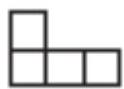
\includegraphics[max width=\textwidth, center]{2024_11_21_0c70f93de31c83ffd191g-1}
  \item Na podstawie \(A B\) trapezu \(A B C D(|A B|>|C D|)\) wyznaczono taki punkt \(E\), że czworokąt \(A E C D\) jest równoległobokiem. Przekątna \(B D\) przecina odcinki \(C A\) i \(C E\) odpowiednio w punktach \(F\) i \(G\). Odcinki \(D G\) i \(B F\) są równej długości. Uzasadnij, że \(\frac{|A B|}{|C D|}=\frac{1+\sqrt{5}}{2}\).\\
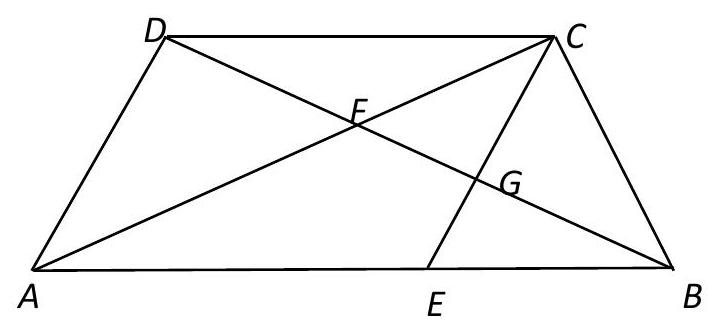
\includegraphics[max width=\textwidth, center]{2024_11_21_0c70f93de31c83ffd191g-1(1)}
\end{enumerate}

\end{document}